\section{The Algorithm}
The algorithm of the FDTD method first introduced by Yee in 1966 swiftly became one of most popular numerical
electromagnetics approach after '80s due to the blooming of computer industry. By discretizing Maxwell's curl equations
via central-difference approximations in time and space partial derivatives, Maxwell's divergence equations are
automatically satisfied and transient behavior of electromagnetics wave are offered.

Primitve Maxwell's equations are elegant enough to describe electromagnetics wave in mathematics. However, for the
purpose of being programmable easily and preventing requiring different equations in simulation for different situation,
the formulas need more symmetric properties in its form. To achieve to goal, some tuning proposed by \textit{Sullivan}
is applied on deriving of update equations to be as general as possible for handling freespace, dielectics, dispersive
material, and even meta-material as well as varieties of PML at the same time.

Moreover, by not only using E and H field but also importing D and B field, material-related terms were collected into
constitutive relations. Apparently it leads to more overhead in every updating loop. However, we acquire more
flexibilities to append more components for complex situations without rewriting the program, being able to concentrate
on modeling of structure for researching. Temporary variables are also reduced due to well integration of formulas to
save the cost of calculation.


\subsection{Finite Difference}
The first thing being concerned is how to discrete space and time in FDTD, in other word, how to turn differential
equations to algerba equations or what the $\partial/\partial t$, $\partial/\partial x$, $\partial/\partial y$,
$\partial/\partial z$ should be. Leapfrog and Semi-Implicit are two possible scheme.
\subsubsection{Explicit Leapfrog Scheme}
Leapfrog scheme is derived from Laylor's series expansion. The adjacent points of arbitrary function $u(x)$ can be
expanded as following.
\begin{equation}
  u(x_i+\Delta x) = u|_{x_i} + 
  \Delta x\cdot\left.\frac{\partial u}{\partial x}\right|_{x_i} + 
  \frac{(\Delta x)^2}{2}\cdot\left.\frac{\partial ^2 u}{\partial x^2}\right|_{x_i} + 
  \frac{(\Delta x)^3}{6}\cdot\left.\frac{\partial ^3 u}{\partial x^3}\right|_{x_i} + ...
\end{equation}
\begin{equation}
  u(x_i-\Delta x) = u|_{x_i} -
  \Delta x\cdot\left.\frac{\partial u}{\partial x}\right|_{x_i} + 
  \frac{(\Delta x)^2}{2}\cdot\left.\frac{\partial ^2 u}{\partial x^2}\right|_{x_i} -
  \frac{(\Delta x)^3}{6}\cdot\left.\frac{\partial ^3 u}{\partial x^3}\right|_{x_i} + ...
\end{equation}
First order derivatives can be retrieved by performing subtracting.
\begin{equation}
  u(x_i+\Delta x) - u(x_i-\Delta x) = 2\Delta x\cdot\left.\frac{\partial u}{\partial x}\right|_{x_i}+...
\end{equation}
\begin{equation}
  \left.\frac{\partial u}{\partial x}\right|_{x_i} = \frac{u(x_i+\Delta x) - u(x_i-\Delta x)}{2\Delta x} = \frac{u^{i+1} - u^{i-1}}{2\Delta x} + O[(\Delta x)^3]
\end{equation}
And performing summing can earn second order derivatives.
\begin{equation}
  u(x_i+\Delta x) + u(x_i-\Delta x) = \left.2u\right|_{x_i} + (\Delta x)^2\cdot\left.\frac{\partial ^2 u}{\partial x^2}\right|_{x_i} + ...
\end{equation}
\begin{equation}
  \left.\frac{\partial^2 u}{\partial x^2}\right|_{x_i} = \frac{u(x_i+\Delta x) - 2u(x_i) + u(x_i-\Delta x)}{(\Delta x)^2} = \frac{u^{i+1} - 2u^i + u^{i-1}}{(\Delta x)^2} % + O[(\Delta x)^2]
\end{equation}


\subsubsection{Semi-Implicit Scheme}
Semi-Implicit is a scheme requiring only two adjacent point, which is similar to calculation of slope. First order
derivatives can be showed as following.
\begin{equation}
  \left.\frac{\partial u}{\partial x}\right|_{x_i} = \frac{u(x_i+\Delta x) - u(x_i)}{\Delta x}
\end{equation}





\subsection{The Update Equations}
Following is the most well-known form of Maxwell's Equations\index{Maxwell's Equations} in time domain, for getting
sysmetrical form and handling metamaterial, novel magnetic current $M$ was added into Faraday's Law.
\begin{gather}
  \label{eq:maxwell}
  \begin{array}{@{}rclr@{}}
    \nabla \cdot \epsilon E & = & \rho_{\nu} & \mathrm{(Gaussian's\ Law)}\\
    \nabla \times E & = & {\displaystyle -\mu\frac{\partial H}{\partial t} - M} & \mathrm{(Faraday's\ Law)}\\
    \nabla \cdot \mu H & = & 0 & \\
    \nabla \times H & = &  {\displaystyle \epsilon\frac{\partial E}{\partial t} + J} & \mathrm{(Amp\`ere's\ Law)}
  \end{array}
\end{gather}
Where $J$ and $M$ are electric current and novel magnatic current respectively. Every real world material has its own
definition of $J$ and $M$. For example, for fictitious simple conductive media having constant electric conductivity
$\sigma_e$ and constant magnetic conductivity $\sigma_h$, $J = \sigma_e E$ and $M = \sigma_h H$. For simulating silver,
Drude Model may be applied in definition of $J$. For convenience, following derivation use $J = \sigma_e E$ and $M =
\sigma_h H$.
\begin{gather}
  \epsilon\frac{\partial}{\partial t}E(t) + \sigma_eE(t) = \nabla \times H(t)\\
  \mu\frac{\partial}{\partial t}H(t) + \sigma_hH(t) = - \nabla \times E(t)
\end{gather}
From here, to make equations to be more symmetrical, which would benefit the design of the rest part of algorithm, all
equations should be turned to Gaussian Units. First, $\epsilon_0$ and $\mu_0$ are separated from $\epsilon$ and $\mu$.
\begin{gather}
  \epsilon_r\frac{\partial}{\partial t}E(t) + \frac{\sigma_e}{\epsilon_0}E(t) = \frac{1}{\epsilon_0}\nabla\times H(t)\\
  \mu_r\frac{\partial}{\partial t}H(t) + \frac{\sigma_h}{\mu_0}H(t) = - \frac{1}{\mu_0}\nabla\times E(t)
\end{gather}
Then, following transformation is applied. A tilde symbol (\textasciitilde{}) was appended on each field notation for
distinguishing whether it is in Gaussian Unit or not.
\label{eq:gaussian_unit}
\begin{equation}
  {\displaystyle\widetilde{E} = \sqrt{\frac{\epsilon_0}{\mu_0}}E}
\end{equation}
Finally, the equations becomes
\begin{gather}\label{eq:coordinate_transform}
  \epsilon_r\frac{\partial}{\partial t}\widetilde{E}(t) + \frac{\sigma_e}{\epsilon_0}\widetilde{E}(t) = \frac{1}{\sqrt{\mu_0\epsilon_0}}\nabla\times H(t)\\
  \mu_r\frac{\partial}{\partial t} H(t) + \frac{\sigma_h}{\mu_0}H(t) = - \frac{1}{\sqrt{\mu_0\epsilon_0}}\nabla\times\widetilde{E}(t)
\end{gather}
It does really a magic trick. All of us know $1/\sqrt{\mu_0\epsilon_0}$ are speed of light in freespace and, by Fourier
transform, $\partial/\partial t \rightarrow j\omega$. A fairly beautiful form for implementing was acquired.
\begin{gather}
  j\omega\left(\epsilon_r + \frac{\sigma_e}{j\omega\epsilon_0}\right)\widetilde{E}(\omega) = c_0\ \nabla\times H(\omega)\\
  j\omega\left(\mu_r + \frac{\sigma_h}{j\omega\mu_0}\right)H(\omega) = - c_0\ \nabla\times\widetilde{E}(\omega)
\end{gather}
It could be understanded the two term $\epsilon_r + \sigma_e/j\omega\epsilon_0$ and $\mu_r + \sigma_h/j\omega\mu_0$ are
permittivity and permeability adjusted by character of this specific material. $\epsilon_r^*(\omega)$ and
$\mu_r^*(\omega)$ are given as the formal and general notations for them to adapt different material here. Futhermore,
electric flux ($\widetilde{D}$) and magnetic flux ($\widetilde{B}$) in Gaussian Unit are also redefined.
\begin{gather}
  \frac{\partial}{\partial t}\widetilde{D}(t) = c_0\nabla\times H(t)\label{eq:up_d}\\
  \widetilde{D}(\omega) = \epsilon_r^*(\omega)\widetilde{E}(\omega)\label{eq:cr_d}\\
  \frac{\partial}{\partial t}\widetilde{B}(t) = -c_0\nabla\times\widetilde{E}(t)\label{eq:up_b}\\
  \widetilde{B}(\omega) = \mu_r^*(\omega)H(\omega)\label{eq:cr_b}
\end{gather}
It has obvious benefit from separating constitute relations from updating in time domain rahter than merging constitute
relations into it. The material-related coefficients were collected into constitute relations to handle different
objects, so that no matter what object was changed in region of simulation Eq.\ref{eq:up_d} and Eq.\ref{eq:up_b} keep in
this form.

For example, $\epsilon_r^*(\omega)$ and $\mu_r^*(\omega)$ are just constant $\epsilon_r$ and very small $\mu_r$ in
dielectric. In a simulation mix dielectric and freespace, $\widetilde{E}$ and $H$ could be retrieved via performing
inverse Fourier transform of Eq.\ref{eq:cr_d} and Eq.\ref{eq:cr_b}.
\begin{gather*}
  \widetilde{E}(t) = \frac{\widetilde{D}(t)}{\epsilon_r}\\
  H(t) = \frac{\widetilde{B}(t)}{\mu_r}
\end{gather*}
In the rest part of simulation, freespace, where both $\epsilon_r^*(\omega)$ and $\mu_r^*(\omega)$ are just unit, 
\begin{gather*}
  \widetilde{E}(t) = \widetilde{D}(t)\\
  H(t) = \widetilde{B}(t)
\end{gather*}
As seeing, without changing Eq.\ref{eq:up_d} and Eq.\ref{eq:up_b}, details of material were covered in Eq.\ref{eq:cr_d}
and Eq.\ref{eq:cr_b}.

In general, every material has its own $\epsilon_r^*(\omega)$ varying through whole frequency spectrum due to its own
characters. By applying some mathematical trick Eq.\ref{eq:cr_d} and Eq.\ref{eq:cr_b} can be specialized for different
material to retrieve $\widetilde{E}$ from $\widetilde{D}$ in every time step but Eq.\ref{eq:up_d} and Eq.\ref{eq:up_b}
can be applied directly on every kinds of material. That's the best advanteage separating constitute relations out of
the two update equations in time domain.

\subsubsection{Numerical Dispersion}
By substituting these replacements into Maxwell's Equations, discretized version would be obtained. However, the
procedure also brings about a by-product, numerical-dispersion artifact, which in 3-D can be expressed as
\begin{equation}
  \label{eq:dispersion3d}
  \begin{split}
    \left[\frac{1}{c\Delta t}\sin\left(\frac{\omega\Delta t}{2}\right)\right] = &
    \left[\frac{1}{\Delta x}\sin\left(\frac{k_x\Delta x}{2}\right)\right] + \\ &
    \left[\frac{1}{\Delta y}\sin\left(\frac{k_y\Delta y}{2}\right)\right] +
    \left[\frac{1}{\Delta z}\sin\left(\frac{k_z\Delta z}{2}\right)\right]
  \end{split}
\end{equation}
where $k_x$, $k_y$, $k_z$ are the wavenumber vector and $\omega$ is the numerical angular frequency. For clear view,
Eq.\ref{eq:dispersion3d} was simplified into 1-D
\begin{equation}
  \widetilde{k} = \frac{1}{\Delta x} \cos^{-1} \left\{1+\left(\frac{\Delta x}{c\Delta t}\right)^2\left[\cos(\omega t)-1\right]\right\}
\end{equation}
It gives a explcit commnet to the side effect of discretizing. For better accuracy, numerical dispersion shoulde be
minimized. That is to say, the sampling rate should be raised ($\Delta t \rightarrow 0$) and cell size should be chose
proper. \cite[Taflove 2005]{taflove}


\subsubsection{Courant Condition}
Proper $\Delta x$ could be determined via Courant-Friedrichs-Lewy condition or just Courant conditions which has the
form
\begin{equation}
  \Delta t \le \frac{\Delta x}{\sqrt{n}\cdot c_0}
\end{equation}
where $n$ is the dimension of the simulation. For the convenience of designing mentioned latter, throughout this thesis we
determine $\Delta t$ by
\begin{equation}
  \Delta t = \frac{\Delta x}{2 \cdot c_0}
\end{equation}
It's useful for simplifying update equations.

\subsubsection{Implementation}
Now the most essential update equations were obtained. The next thing is to implement it in real world, which is a three
steps procedure. First of all, extend Eq.\ref{eq:up_d} and Eq.\ref{eq:up_b} in chosen coordinate system. Next, applying
finite difference to replace differential operand. Finally, mapping mathematical coordinate into array of computer
language.

For first step, Our choice is Cartesian coordinate system and the results of extending are shown below.
\begin{equation}
  \overPartialT \widetilde{D}_x = c_0 \curlHxThree \label{eq:up_d_x}
\end{equation}
\begin{equation}
  \overPartialT \widetilde{D}_y = c_0 \curlHyThree \label{eq:up_d_y}  
\end{equation}
\begin{equation}
  \overPartialT \widetilde{D}_z = c_0 \curlHzThree \label{eq:up_d_z}\\  
\end{equation}
\begin{equation}
  \overPartialT \widetilde{B}_x =-c_0 \curlExThree \label{eq:up_b_x}\\  
\end{equation}
\begin{equation}
  \overPartialT \widetilde{B}_y =-c_0 \curlEyThree \label{eq:up_b_y}\\  
\end{equation}
\begin{equation}
  \overPartialT \widetilde{B}_z =-c_0 \curlEzThree \label{eq:up_b_z}
\end{equation}
In the second step, semi-implicit scheme was applied. Yee Mesh in Fig.\ref{fig:yee-grid} is taken as reference.
\begin{center}\label{fig:yee-grid}
  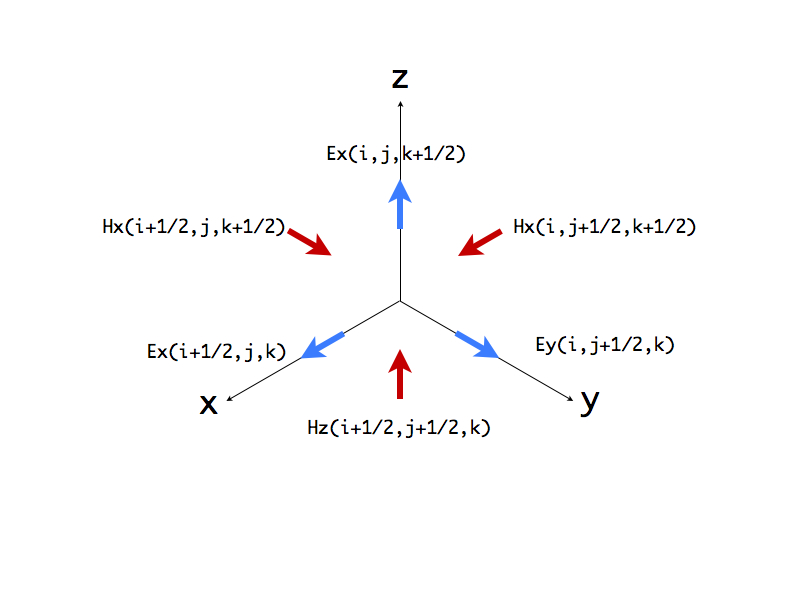
\includegraphics[scale=0.5]{images/yee-grid.jpg}
\end{center}
\begin{equation}
  \begin{split}
    \displaystyle & \frac{\widetilde{D}_x|_{i+\frac{1}{2},j,k}^{n+\frac{1}{2}} - \widetilde{D}_x|_{i+\frac{1}{2},j,k}^{n-\frac{1}{2}}}{\Delta t} = \\
    \displaystyle & c_0\left(\frac{H_z|_{i+\frac{1}{2},j+\frac{1}{2},k}^{n} - H_z|_{i+\frac{1}{2},j-\frac{1}{2},k}^{n}}{\Delta y} - \frac{H_y|_{i+\frac{1}{2},j,k+\frac{1}{2}}^{n} - H_y|_{i+\frac{1}{2},j,k-\frac{1}{2}}^{n}}{\Delta z}\right)\\
  \end{split}
\end{equation}
\begin{equation}
  \begin{split}
    \displaystyle & \frac{\widetilde{D}_y|_{i,j+\frac{1}{2},k}^{n+\frac{1}{2}} - \widetilde{D}_x|_{i,j+\frac{1}{2},k}^{n-\frac{1}{2}}}{\Delta t} = \\
    \displaystyle & c_0\left(\frac{H_x|_{i,j+\frac{1}{2},k+\frac{1}{2}}^{n} - H_x|_{i,j+\frac{1}{2},k-\frac{1}{2}}^{n}}{\Delta z} - \frac{H_z|_{i+\frac{1}{2},j+\frac{1}{2},k}^{n} - H_z|_{i-\frac{1}{2},j+\frac{1}{2},k}^{n}}{\Delta x}\right)\\
  \end{split}
\end{equation}
\begin{equation}
  \begin{split}
    \displaystyle & \frac{\widetilde{D}_z|_{i,j,k+\frac{1}{2}}^{n+\frac{1}{2}} - \widetilde{D}_z|_{i,j,k+\frac{1}{2}}^{n-\frac{1}{2}}}{\Delta t} = \\
    \displaystyle & c_0\left(\frac{H_y|_{i+\frac{1}{2},j,k+\frac{1}{2}}^{n} - H_y|_{i-\frac{1}{2},j,k+\frac{1}{2}}^{n}}{\Delta x} - \frac{H_x|_{i,j+\frac{1}{2},k+\frac{1}{2}}^{n} - H_x|_{i,j-\frac{1}{2},k+\frac{1}{2}}^{n}}{\Delta y}\right)\\
  \end{split}
\end{equation}
\begin{equation}
  \begin{split}
    \displaystyle & \frac{\widetilde{B}_x|_{i,j+\frac{1}{2},k+\frac{1}{2}}^{n+1} - \widetilde{B}_x|_{i,j+\frac{1}{2},k+\frac{1}{2}}^{n}}{\Delta t} = \\
    \displaystyle & - c_0\left(\frac{\widetilde{E}_z|_{i,j+1,k+\frac{1}{2}}^{n+\frac{1}{2}} - \widetilde{E}_z|_{i,j,k+\frac{1}{2}}^{n+\frac{1}{2}}}{\Delta y} - \frac{\widetilde{E}_y|_{i,j+\frac{1}{2},k+1}^{n+\frac{1}{2}} - \widetilde{E}_y|_{i,j+\frac{1}{2},k}^{n+\frac{1}{2}}}{\Delta z}\right)\\
  \end{split}
\end{equation}
\begin{equation}
  \begin{split}
    \displaystyle & \frac{\widetilde{B}_y|_{i+\frac{1}{2},j,k+\frac{1}{2}}^{n+1} - \widetilde{B}_y|_{i+\frac{1}{2},j,k+\frac{1}{2}}^{n}}{\Delta t} = \\
    \displaystyle & - c_0\left(\frac{\widetilde{E}_x|_{i+\frac{1}{2},j,k+1}^{n+\frac{1}{2}} - \widetilde{E}_x|_{i+\frac{1}{2},j,k}^{n+\frac{1}{2}}}{\Delta z} - \frac{\widetilde{E}_z|_{i+1,j,k+\frac{1}{2}}^{n+\frac{1}{2}} - \widetilde{E}_z|_{i,j,k+\frac{1}{2}}^{n+\frac{1}{2}}}{\Delta x}\right)\\
  \end{split}
\end{equation}
\begin{equation}
  \begin{split}
    \displaystyle & \frac{\widetilde{B}_z|_{i+\frac{1}{2},j+\frac{1}{2},k}^{n+1} - \widetilde{B}_z|_{i+\frac{1}{2},j+\frac{1}{2},k}^{n}}{\Delta t} = \\
    \displaystyle & - c_0\left(\frac{\widetilde{E}_y|_{i+1,j+\frac{1}{2},k}^{n+\frac{1}{2}} - \widetilde{E}_y|_{i,j+\frac{1}{2},k}^{n+\frac{1}{2}}}{\Delta x} - \frac{\widetilde{E}_x|_{i+\frac{1}{2},j+1,k}^{n+\frac{1}{2}} - \widetilde{E}_x|_{i+\frac{1}{2},j,k}^{n+\frac{1}{2}}}{\Delta y}\right)
  \end{split}
\end{equation}
Throughout this thesis, we use regular grid, that is, $\Delta x = \Delta y = \Delta z$. That means we could rewrite update equations as
\begin{equation}\label{eq:dx3d}
  \begin{split}
    \widetilde{D}_x|_{i+\frac{1}{2},j,k}^{n+\frac{1}{2}} & = \widetilde{D}_x|_{i+\frac{1}{2},j,k}^{n-\frac{1}{2}}\\
    & + \frac{c_0\Delta t}{\Delta x}\left(H_z|_{i+\frac{1}{2},j+\frac{1}{2},k}^{n} - H_z|_{i+\frac{1}{2},j-\frac{1}{2},k}^{n} - H_y|_{i+\frac{1}{2},j,k+\frac{1}{2}}^{n} + H_y|_{i+\frac{1}{2},j,k-\frac{1}{2}}^{n}\right)
  \end{split}
\end{equation}
\begin{equation}
  \begin{split}
    \widetilde{D}_y|_{i,j+\frac{1}{2},k}^{n+\frac{1}{2}} & = \widetilde{D}_x|_{i,j+\frac{1}{2},k}^{n-\frac{1}{2}}\\
    & + \frac{c_0\Delta t}{\Delta x}\left(H_x|_{i,j+\frac{1}{2},k+\frac{1}{2}}^{n} - H_x|_{i,j+\frac{1}{2},k-\frac{1}{2}}^{n} - H_z|_{i+\frac{1}{2},j+\frac{1}{2},k}^{n} + H_z|_{i-\frac{1}{2},j+\frac{1}{2},k}^{n}\right)
  \end{split}
\end{equation}
\begin{equation}\label{eq:dz3d}
  \begin{split}
    \widetilde{D}_z|_{i,j,k+\frac{1}{2}}^{n+\frac{1}{2}} & = \widetilde{D}_z|_{i,j,k+\frac{1}{2}}^{n-\frac{1}{2}}\\
    & + \frac{c_0\Delta t}{\Delta x}\left(H_y|_{i+\frac{1}{2},j,k+\frac{1}{2}}^{n} - H_y|_{i-\frac{1}{2},j,k+\frac{1}{2}}^{n} - H_x|_{i,j+\frac{1}{2},k+\frac{1}{2}}^{n} + H_x|_{i,j-\frac{1}{2},k+\frac{1}{2}}^{n}\right)
  \end{split}
\end{equation}
\begin{equation}\label{eq:bx3d}
  \begin{split}
    \widetilde{B}_x|_{i,j+\frac{1}{2},k+\frac{1}{2}}^{n+1} & = \widetilde{B}_x|_{i,j+\frac{1}{2},k+\frac{1}{2}}^{n}\\
    & - \frac{c_0\Delta t}{\Delta x}\left(\widetilde{E}_z|_{i,j+1,k+\frac{1}{2}}^{n+\frac{1}{2}} - \widetilde{E}_z|_{i,j,k+\frac{1}{2}}^{n+\frac{1}{2}} - \widetilde{E}_y|_{i,j+\frac{1}{2},k+1}^{n+\frac{1}{2}} - \widetilde{E}_y|_{i,j+\frac{1}{2},k}^{n+\frac{1}{2}}\right)
  \end{split}
\end{equation}
\begin{equation}\label{eq:by3d}
  \begin{split}
    \widetilde{B}_y|_{i+\frac{1}{2},j,k+\frac{1}{2}}^{n+1} & = \widetilde{B}_y|_{i+\frac{1}{2},j,k+\frac{1}{2}}^{n}\\
    & - \frac{c_0\Delta t}{\Delta x}\left(\widetilde{E}_x|_{i+\frac{1}{2},j,k+1}^{n+\frac{1}{2}} - \widetilde{E}_x|_{i+\frac{1}{2},j,k}^{n+\frac{1}{2}} - \widetilde{E}_z|_{i+1,j,k+\frac{1}{2}}^{n+\frac{1}{2}} - \widetilde{E}_z|_{i,j,k+\frac{1}{2}}^{n+\frac{1}{2}}\right)
  \end{split}
\end{equation}
\begin{equation}
  \begin{split}
    \widetilde{B}_z|_{i+\frac{1}{2},j+\frac{1}{2},k}^{n+1} & = \widetilde{B}_z|_{i+\frac{1}{2},j+\frac{1}{2},k}^{n}\\
    & - \frac{c_0\Delta t}{\Delta x}\left(\widetilde{E}_y|_{i+1,j+\frac{1}{2},k}^{n+\frac{1}{2}} - \widetilde{E}_y|_{i,j+\frac{1}{2},k}^{n+\frac{1}{2}} - \widetilde{E}_x|_{i+\frac{1}{2},j+1,k}^{n+\frac{1}{2}} - \widetilde{E}_x|_{i+\frac{1}{2},j,k}^{n+\frac{1}{2}}\right)
  \end{split}
\end{equation}
This is complete update equations derived for 3D cases. Also, $c_0\Delta t/\Delta x$ can be simply written as 0.5 for
our convenience of Courant condition. For short, the curl part in parentheses and be denoted as $curl\_hx$
(Eq.\ref{eq:dx3d}), $curl\_ex$ (Eq.\ref{eq:bx3d}) and so on.

Finally, non-integer index number can be mapped into array of computer language via
\begin{equation}
  k+\frac{1}{2}\rightarrow k\quad \mathrm{and} \quad
  k-\frac{1}{2}\rightarrow k-1
\end{equation}
Here is the transformation to pseudo code
\begin{code}
  dx[i,j,k] += 0.5 * ( self.hz[i,j,k] - self.hz[i,j-1,k] 
                     - self.hy[i,j,k] + self.hy[i,j,k-1] )
  dy[i,j,k] += 0.5 * ( self.hx[i,j,k] - self.hx[i,j,k-1] 
                     - self.hz[i,j,k] + self.hz[i-1,j,k] )
  dz[i,j,k] += 0.5 * ( self.hy[i,j,k] - self.hy[i-1,j,k] 
                     - self.hx[i,j,k] + self.hx[i,j-1,k] )
  
  bx[i,j,k] -= 0.5 * ( self.ez[i,j+1,k] - self.ez[i,j,k] 
                     - self.ey[i,j,k+1] + self.ey[i,j,k] )
  by[i,j,k] -= 0.5 * ( self.ex[i,j,k+1] - self.ex[i,j,k] 
                     - self.ez[i+1,j,k] + self.ez[i,j,k] )
  bz[i,j,k] -= 0.5 * ( self.ey[i+1,j,k] - self.ey[i,j,k] 
                     - self.ex[i,j+1,k] + self.ex[i,j,k] )
\end{code}




\subsection{Reduction to One Dimensions}
There are three selections to choose a one dimension EM string: $\mathrm{TEM_x}$ ($\mathrm{E_{y}}$, $\mathrm{H_{z}}$,
$\mathrm{k_x}$), $\mathrm{TEM_y}$ ($\mathrm{E_z}$, $\mathrm{H_x}$, $\mathrm{k_y}$), and $\mathrm{TEM_z}$
($\mathrm{E_x}$, $\mathrm{H_y}$, $\mathrm{k_z}$). Similarly, $\mathrm{TEM_z}$ is the default choice when saying
TEM. Following the definition of TEM, Eq.\ref{eq:up_d_x} and Eq.\ref{eq:up_b_y} were picked out for reduction of 1-D
case. The choice implies
\begin{displaymath}
  \frac{\partial}{\partial x} \rightarrow 0\quad \mathrm{and} \quad
  \frac{\partial}{\partial y} \rightarrow 0
\end{displaymath}
apply these conditions on Eq.\ref{eq:up_d_x} and Eq.\ref{eq:up_b_y}, they becomes
\begin{gather}
  \frac{\partial}{\partial t}\widetilde{D}_x = \frac{1}{\sqrt{\mu_0\epsilon_0}}\left( - \frac{\partial H_y}{\partial z}\right)\\
  \frac{\partial}{\partial t}\widetilde{B}_y =-\frac{1}{\sqrt{\mu_0\epsilon_0}}\left(\frac{\partial \widetilde{E}_x}{\partial z} \right)
\end{gather}
The only two equations are time domain equation for 1-D. Following the same procedure as 3-D to discrete
\begin{gather}
  \widetilde{D}_x|_k^{n+\frac{1}{2}} = \widetilde{D}_x|_k^{n-\frac{1}{2}} - \frac{c_0\Delta t}{\Delta z}\left( H_y|_{k+\frac{1}{2}}^n - H_y|_{k-\frac{1}{2}}^n \right)\\
  \widetilde{B}_y|_{k+\frac{1}{2}}^{n+1} = \widetilde{B}_y|_{k+\frac{1}{2}}^{n} - \frac{c_0\Delta t}{\Delta z}\left( \widetilde{E}_x|_{k+1}^{n+\frac{1}{2}} - \widetilde{E}_x|_{k}^{n+\frac{1}{2}} \right)
\end{gather}



\subsection{Reduction to Two Dimensions}
There are 6 selections for us to choose a two dimensions EM plane: $\mathrm{TM_{x}} $, $\mathrm{TE_{x}}$,
$\mathrm{TM_{y}}$, $\mathrm{TE_{y}}$, $\mathrm{TM_{z}}$, $\mathrm{TE_{z}}$. By default, the choice in this thesis follow
the book of Taflove using $\mathrm{TM_{z}}$ ($\mathrm{H_x}$, $\mathrm{H_y}$, and $\mathrm{E_z}$) and $\mathrm{TE_{z}}$
($\mathrm{E_x}$, $\mathrm{E_y}$, and $\mathrm{H_z}$) as convention when saying TM and TE. Both $\mathrm{TM_z}$ and
$\mathrm{TE_z}$ should satisfy.
\begin{displaymath}
  \frac{\partial}{\partial z} \rightarrow 0
\end{displaymath}
When applying the condition, $\mathrm{TM_z}$ becomes
\begin{displaymath}
  \frac{\partial}{\partial t}\widetilde{D}_z = c_0 \curlHzTwo
\end{displaymath}
\begin{displaymath}
  \frac{\partial}{\partial t}\widetilde{B}_x =-c_0 \curlExTwo
\end{displaymath}
\begin{displaymath}
  \frac{\partial}{\partial t}\widetilde{B}_y =-c_0 \curlEyTwo
\end{displaymath}
and $\mathrm{TE_z}$ becomes
\begin{displaymath}
    \frac{\partial}{\partial t}\widetilde{B}_z =-c_0 \curlEzTwo
\end{displaymath}
\begin{displaymath}
  \frac{\partial}{\partial t}\widetilde{D}_x = c_0 \curlHxTwo
\end{displaymath}
\begin{displaymath}
  \frac{\partial}{\partial t}\widetilde{D}_y = c_0 \curlHyTwo
\end{displaymath}
Note they are two independent sets because they don't use component of each other for updating itself. For less overhead
of memory, we can define two class \texttt{TMPlane} having first three methods and \texttt{TEPlane} having the
rest. However, it would be more convenient to handle two kinds of polarization in one class via gathering all eqautions
as methods of one class \texttt{Plane} rather than defining two class. The last way also has advantage to simulate
circle polarization.

Again, Following identical procedure to discretize, we would obtain the equations for computing
\begin{displaymath}
  \frac{\widetilde{D}_z|_{i,j}^{n+\frac{1}{2}}-\widetilde{D}_z|_{i,j}^{n+\frac{1}{2}}}{\Delta t} =
  c_0 \left(\frac{H_y|_{i+\frac{1}{2},j}^{n} - H_y|_{i-\frac{1}{2},j}^n}{\Delta x} - \frac{H_x|_{i,j+\frac{1}{2}}^{n} - H_x|_{i,j-\frac{1}{2}}^{n}}{\Delta y}\right)
\end{displaymath}
\begin{displaymath}
  \frac{\widetilde{B}_x|_{i,j+\frac{1}{2}}^{n+1} - \widetilde{B}_x|_{i,j+\frac{1}{2}}^{n}}{\Delta t} = 
  - c_0\left(\frac{\widetilde{E}_z|_{i,j+1}^{n+\frac{1}{2}} - \widetilde{E}_z|_{i,j}^{n+\frac{1}{2}}}{\Delta y}\right)
\end{displaymath}
\begin{displaymath}
  \frac{\widetilde{B}_y|_{i+\frac{1}{2},j}^{n+1} - \widetilde{B}_y|_{i+\frac{1}{2},j}^{n}}{\Delta t} =
  - c_0\left( - \frac{\widetilde{E}_z|_{i+1,j}^{n+\frac{1}{2}} - \widetilde{E}_z|_{i,j}^{n+\frac{1}{2}}}{\Delta x}\right)
\end{displaymath}
\begin{displaymath}
  \frac{\widetilde{B}_z|_{i+\frac{1}{2},j+\frac{1}{2}}^{n} - \widetilde{B}_z|_{i+\frac{1}{2},j+\frac{1}{2}}^{n}}{\Delta t} =
  c_0\left(\frac{\widetilde{E}_y|_{i+1,j+\frac{1}{2}}^{} - \widetilde{E}_y|_{i,j+\frac{1}{2}}^{}}{\Delta x} - \frac{\widetilde{E}_x|_{i+\frac{1}{2},j+1}^{} - \widetilde{E}_x|_{i+\frac{1}{2},j}^{}}{\Delta y}\right)
\end{displaymath}
\begin{displaymath}
  \frac{\widetilde{D}_x|_{i+\frac{1}{2},j}^{n+\frac{1}{2}} - \widetilde{D}_x|_{i+\frac{1}{2},j}^{n-\frac{1}{2}}}{\Delta t} =
  c_0\left(\frac{H_z|_{i+\frac{1}{2},j+\frac{1}{2}}^{n} - H_z|_{i+\frac{1}{2},j-\frac{1}{2}}^{n}}{\Delta y} - \right)
\end{displaymath}
\begin{displaymath}
  \frac{\widetilde{D}_y|_{i,j+\frac{1}{2}}^{n+\frac{1}{2}} - \widetilde{D}_x|_{i,j+\frac{1}{2}}^{n-\frac{1}{2}}}{\Delta t} =
  c_0\left( - \frac{H_z|_{i+\frac{1}{2},j+\frac{1}{2}}^{n} - H_z|_{i-\frac{1}{2},j+\frac{1}{2}}^{n}}{\Delta x}\right)
\end{displaymath}


